% "Станет проще"

\documentclass[a4paper,12pt]{article} % тип документа

% report, book

%  Русский язык
% процент означает комментарий

\usepackage[T2A]{fontenc}			% кодировка
\usepackage[utf8]{inputenc}			% кодировка исходного текста
\usepackage[english,russian]{babel}	% локализация и переносы
\usepackage{wrapfig}

% Буквенные списки
\renewcommand{\theenumi}{(\asbuk{enumi})}
\renewcommand{\labelenumi}{\asbuk{enumi})}



% Математика
\usepackage{amsmath,amsfonts,amssymb,amsthm,mathtools} 
\usepackage{wasysym}

%Заговолок
%------------------------------------------------------

\newenvironment{bottompar}{\par\vspace*{\fill}}{\clearpage}

\begin{document} % начало документа


\begin{titlepage}
\newcommand{\HRule}{\rule{\linewidth}{0.5mm}} % Defines a new command for the horizontal lines, change thickness here

\center % Center everything on the page
 
\textsc{
\Large Московский\\[-0.2cm]Физико-Технический Институт\\[0.1cm]\large (государственный университет)}\\[1.5cm] % Name of your university/college
\textsc{\Large Кафедра общей физики}\\[0.2cm] % Major heading such as course name
\textsc{\large Электричество и магнетизм:\\ лабораторный практикум}\\[0.5cm]
\textsc{\large Лабораторная работа \textnumero 3.6.1} % Minor heading such as course title

\HRule
\\[0.1cm]
{ \large \bfseries Спектральный анализ 
\\[0.0cm] электрических сигналов} % Title of your document
\HRule
\\[1.5cm]


\begin{center} % just for vertical spacing and killing indent
\begin{tabular*}{\textwidth}{@{}l@{\extracolsep{\fill}}r@{}}
\textbf{Студент}  & \textbf{Преподаватель} \\
Соколов Вадим  & Александр Аркадьевич \\
718 группа & Нозик \\
\end{tabular*}
\end{center}

%\begin{flushright} \large
	%\textsf{Преподаватель}\\[0.1cm]
	%Нозик\\ Александр Аркадьевич
%\end{flushright}

\begin{bottompar}
	\begin{center}
		
\includegraphics[width = 80 mm]{Images/logo.jpg}
	\end{center}
	{\large \today}

\end{bottompar}
\vfill
\end{titlepage}

%------------------------------------------------------

\newpage

\subsection*{Цель работы}
.

\subsection*{Оборудование}
Двухлучевой сканирующий спектрофотометр Shimadzu UV-1800; ячейка, наполненная \(N_2O_4\).

\begin{center}
Введение
\end{center}

Положение химического равновесия может быть с высокой точностью рассчитано на основании термодинамических функций участников процесса. Такие расчеты являются основой решения множества важных практических задач. С другой стороны, термодинамические функции реакций чаще всего получают именно из данных по химическим равновесиям, хотя есть и другие экспериментальные источники, например, калориметрия, спектроскопия, теплоемкость и др. Специалистам разных областей химии, биологии, физики и техники необходимо свободно решать как прямые, так и обратные задачи химических равновесий.
В настоящей работе предлагается познакомиться с этими методами на примере равновесия диссоциации

\begin{equation}\label{chem}
N_2O_4 \Leftrightarrow 2NO_2
\end{equation}
в газовой фазе.

Для измерения степени диссоциации в данной работе используется интенсивное поглощение молекулами NO2 света в видимой области спектра. Измерения проводят при разных температурах, получая температурную зависимость константы равновесия \eqref{chem}, которую анализируют в рамках имеющейся теории.

\begin{center}
{ \LARGE Tеоретические основы}
\end{center}
Условие химического равновесия, как известно, записывается в форме равенства нулю изменения термодинамического потенциала системы в ходе реакции, т. е.
\begin{equation}
 \Delta G_{T,p}  = 0
\end{equation}	

Согласно определению

\begin{equation}
 \Delta G_{T,p}  = \sum {(\frac{\partial G}{\partial n_i})_{T,p} dn_i = \sum {\mu_i dn_i}  }
\end{equation}	
где \(n_i\), — число молей i-го компонента системы 1, а \(\mu_i\), — его химический потенциал, являющийся мерой влияния данного вещества на термодинамическое состояние системы. Уравнение (3) записано при условии постоянства концентраций всех компонентов системы, кроме i-го. Зависимость химического потенциала идеального газа от давления дается формулой

\begin{equation}
 \mu_i = \mu_i^0 + RT \ln{p_i}
\end{equation}
в которой \( \mu_i^0 \) - стандартный химический потенциал i-го компонента при 1 атм.
Если исключительно для простоты записи последующих уравнений представить равновесие (1) в форме

\begin{equation}\label{BA}
 B \Leftrightarrow 2A
\end{equation}
то на основании приведенных выше соотношений условие равновесия реакции \eqref{BA} можно записать в виде

\begin{equation}
 2 \mu_A^0 + RT \ln{p_A^2} - \mu_B^0 - RT \ln{p_B} = 0,
\end{equation}
и после несложного преобразования получим выражение

\begin{equation} \label{RT}
 -RT \ln(p_A^2 / p_B) = 2 \mu_A^0 - \mu_B^0
\end{equation}

в котором комбинация давлений газов в равновесной системе, стоящая в скобках, соответствует константе равновесия

\begin{equation} \label{Koeff}
 K_p = p_A^2 / p_B
\end{equation}
Подставляя \eqref{Koeff} в \eqref{RT}, получим выражение
\begin{equation}
 -RT \ln(K_p) =  2 G_A^0 - G_B^0 = \Delta G^0,
\end{equation}
являющееся условием химического равновесия. В нем скрыта размерность константы равновесия, которая связана с выбором стандартного состояния. Можно записать

\begin{equation}
 \Delta G^0 = -RT ln(K_p / K_p^0)
\end{equation}
причем в стандартном состоянии \(K_p^0\) в скобке равно единице в размерности этого состояния в соответствующей степени. Например, для газов в качестве стандартного состояния в большинстве случаев используют 1 атм, так что в рассматриваемом равновесии \(K_p\) и \(K_p^0\) выражены в атм.
Изменение термодинамического потенциала, в свою очередь, связано с изменениями энтальпии и энтропии в реакции соотношением:

\begin{equation}
 \Delta G^0 = \Delta H^0 - T \Delta S^0
\end{equation}

Величина каждой из составляющих его функций зависит от температуры согласно приближенным уравнениям:

\begin{equation}
 \Delta H_T^0 = \Delta H_{298}^0 + \Delta c_p \Delta T
\end{equation}

\begin{equation}
 \Delta S_T^0 = \Delta S_{298}^0 + \Delta c_p \Delta \ln{T}
\end{equation}
в которых \(\Delta r c_p\) представляет собой разность теплоёмкостей продуктов и исходных веществ, а приращение Т и lnТ отсчитываются от стандартной температуры 298,15 К. Для относительно узких температурных интервалов этими зависимостями можно пренебречь, что приводит к окончательным соотношениям:

\begin{equation}
 \Delta G_T^0 = \Delta H_{298}^0 - T \Delta S_{298}^0
\end{equation}

\begin{equation}
 RT \ln K_p = - \Delta G_T^0 = -\Delta H_{298}^0 + T \Delta S_{298}^0
\end{equation}
которыми предлагается пользоваться в дальнейших расчетах.
	
В практически более удобной записи выражения (8) для константы равновесия реакции (1) в форме (5) используют степень диссоциации \(\alpha\). Предположим, что в замкнутую систему объемом \(V_0\) введено \(n_0\) молей газа В, так что суммарная концентрация обоих газов, выраженная в молях В и независящая от Т, составляет

\begin{equation}
 C_0 = n_0 /V_0
\end{equation}

а их полное давление:

\begin{equation}
 p_0 = RT \cdot C_0
\end{equation}

Такое давление имела бы система при температуре Т в условиях полной диссоциации. В иных условиях парциальные давления газов будут определяться уравнением материального баланса:

\begin{equation}
 p_0 = 2p_B + p_A,
\end{equation}

поскольку каждая молекула В содержит две молекулы А.
Если степень диссоциации определить как

\begin{equation}
 \alpha = \frac{N_A}{N_0}	
\end{equation}

Где $N_0$ - количество всех молекул $N_2 O_4$, а $N_A$ - количество продиссоциировавших молекул $N_2 O_4$.

Тогда с учётом формулы (17) получим для давлений газов:

\begin{equation}
 p(N_2 O_4)  = (1 - \alpha) \cdot C_0 RT,
\end{equation}


\begin{equation}
p(N O_2)  = 2\alpha \cdot C_0 RT.
\end{equation}


Подставляя (20) и (21) в (8), получим выражение для константы равновесия диссоциации:

\begin{equation}
K_p = \frac{4 \alpha^2}{1- \alpha}\cdot C_0 RT.
\end{equation}



\subsection*{Методика измерений}

Исследование степени диссоциации газа проводится с помощью спектрофотометра Shimadzu UV-1800, который позволяет проводить измерения оптической плотности ячейки в целом диапазоне волн(от 400 до 500 нм в нашей работе)с заданным шагом(0,1 нм в нашей работе) и при разных температурах(от 30 $^\circ$C до 80 $^\circ$C в нашей работе). Обозначим такой набор исходных данных через $D_(ij) = D(\Lambda_i;T_j)$, где длины волн и температуры намеруются индексами i и j соответственно. Предполагается, что выполняется закон Бугера-Ламберта-Бэра о том, что эта оптическая плотность представима в виде  линейной комбинации двух составляющих, зависящих только от длины волны и только от температуры:

\begin{equation}
 D_(ij) =D_o + 2\alpha_jC_o \cdot \epsilon_i \cdot l,
\end{equation}

Где $C_o$ - концентрация недиссоциированного $N_2 O_4$, $\alpha_j$ - степень диссоциации, $D_o$ - оптическая плотность пустой ячейки, $\epsilon_i$ -  коэффицент молярного поглощения(коэффицент экстинкции), показывающий, насколько сильно вещество поглощает свет на заданной длине волны. Очевидно, что коэффицент экстинкции не зависит от температуры, а концентрация $NO_2$ - от длины волны, на которой проводятся измерения. 

\begin{figure}[h]
	\begin{center}
		\begin{minipage}{0.45 \linewidth}
			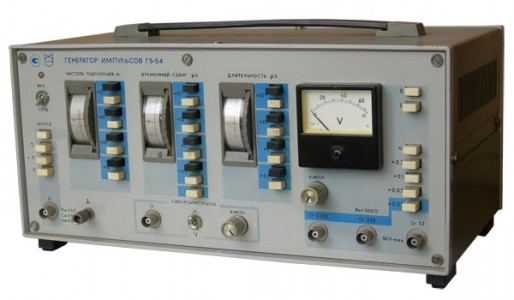
\includegraphics[width = 7cm]{Images/Producer G5-54.jpg}
		\end{minipage}
		\qquad
		\begin{minipage}{0.45 \linewidth}
			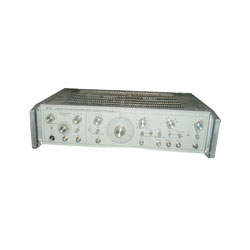
\includegraphics[width = 7cm]{Images/Producer G6-34.jpg}
		\end{minipage}
	\end{center}
	\caption{Cхема установки}
\end{figure}


\begin{enumerate}
	\item Подготовка установки
	\item Установка температуры
	\item Измерение оптической плотности ячейки
\end{enumerate}


\emph{Подготовка установки}

Очистим от загрязнений поверхность ячейки влажной тканью. Откалибруем фотоспектрометр.


\begin{figure}
	\begin{minipage}{0.45 \linewidth}
		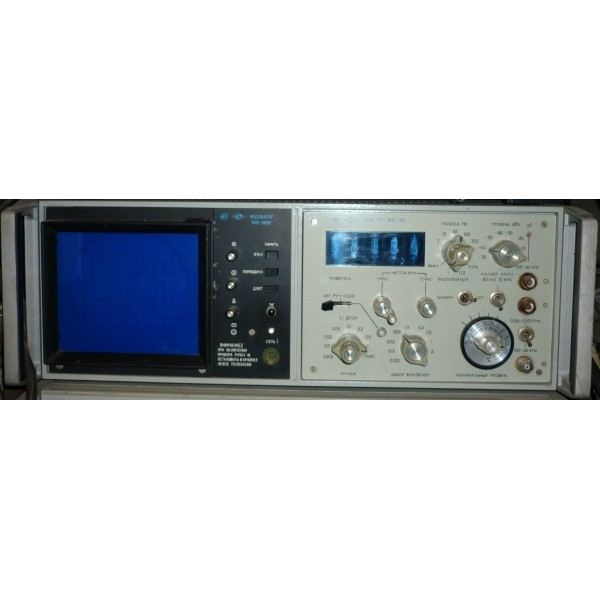
\includegraphics[width = 7cm]{Images/Spectral analyzer SK4-56.jpg}
	\end{minipage}
	\caption{установка ячейки}
\end{figure}

\emph{Установка температуры}
Включив термостат, установим на нем начальную температуру (30 $^\circ$C). Дождемся установления равновесного состояния в системе.

\emph{Измерение оптической плотности ячейки}
Проведем измерение оптической плотности ячейки при помощи фотоспектрографа в режиме Spectrum. Повторим пункты б) и в) , увеличивая температуру ячейки на 5 $^\circ$C. Получим температурную зависимость оптической плотности газа в ячейке с максимальной температурой 80 $^\circ $C .

Из уравнения (15) получим конечную расчётную формулу:

\begin{equation}
\ln K_p = \ln \frac{ \alpha_j^2}{1 - \alpha_j} + \ln T + \ln (4C_0 R) = \frac{-\Delta H}{RT} + \frac{\Delta S}{R}
\end{equation}

Где $\alpha_j$ - это степень диссоциации газа при конкретном значении температуры $T_j$. 

Следовательно, функция $y_j =  \ln \frac{ \alpha_j^2}{1 - \alpha_j} + \ln T_j $ должна линейно зависеть от обратной температуры $x_j = 1/T_j$. 
Попробуем исследовать эту зависимость, используя закон Бугера-Ламберта-Бэра(формула(23)): 


\begin{equation}
D(ij) =D_o + 2\alpha_jC_o \cdot \epsilon_i \cdot l
\end{equation}
\begin{equation}
D(ij) - D(i1) =2(\alpha_j - \alpha_1)C_o \cdot \epsilon_i\cdot l
\end{equation}
\begin{equation}
D(i2) - D(1j) =2( \alpha_2 - \alpha_j)C_o \cdot \epsilon_i \cdot l
\end{equation}
Из уравнений (26)(27) выразим величину $\Delta$, зависящую только от температуры:
\begin{equation}
\Delta_{ij} = \frac{D_{ij} - D_{i1}}{D_{i2} - D_{ij}} = \frac{\alpha_{j} - \alpha_{1}}{\alpha_{2} - \alpha_{j}} = \Delta_{j}
\end{equation}
\begin{equation}
\alpha_j = \frac{\alpha_1 + \Delta_{j}\alpha_2}{1 + \Delta_{j}}
\end{equation}
Мерой линейности служит коэффицент корреляции $R = \frac{cov(x;y)}{\sigma_x\sigma_y}$: чем ближе он по модулю к единице, тем больше проявляется линейная зависимость между  x и y. Поскольку у является параметрической функцией от $\alpha_1$ и $\alpha_2$, то коэффицент корреляции сам получается функцией от этих параметров. С помощью матпакета Excel можно подобрать такие значения $\alpha_1$ и $\alpha_2$, чтобы максимизировать коэффициент корреляции. Для большей точности может максимизировать сумму $\sum_{i}R_i^2(x, y)$ коэффицентов корреляции на всех длинах волн, для которых были проведены измерения(в нашей работе используется 751 значение длин волн в диапазоне от 425 до 500 нм.


\begin{figure}[h!]
\begin{center}

\includegraphics[width=1.0\textwidth]{Images/logo.jpg}
\end{center}
\caption{график значений энтальпий для различных длин волн} \label{dz1}
\end{figure}

\begin{figure}[h!]
\begin{center}

\includegraphics[width=1.2\textwidth]{Images/logo.jpg}
\end{center}
\caption{вычисление значения степени диссоциации} \label{dz1}
\end{figure}


В результате будут получены степени диссоциации $N_2O_4$ при опорных температурах, угол наклона a зависимости $\ln K_c(1/T_j)$:
\begin{equation}
a = \frac{ <xy> - <x><y>}{<x^2> - <x>^2} = -\frac{\Delta H}{R}
\end{equation}
Отсюда сразу получается изменение энтальпии реакции диссоциации(). Оно отличается от табличного на ($\Delta H_{табл} = 57,27$ кДж/моль).

\subsection*{Погрешности}

Найдём теперь погрешность для полученного значения $\Delta H$.
С помощью метода наименьших квадратов (МНК) найдём значение $\sigma_{\Delta H} = 2.12$ кДж/моль. Относительная погрешность составила примерно $\sigma_{rdm} = 4 \%$.


Так же оценим приборную погрешность.
Для термостата из паспорта прибора погрешность равняется $\sigma_{app} = 3 \%$.
У спектрофотометра Shimadzu UV-1800 погрешность установки длины волны не более $0.1 \%$. 

Посчитаем абсолютную погрешность как:
\begin{equation}
\sigma_{\Delta H} = \sqrt{\sigma_{app}^2+\sigma_{rdm}^2}
\end{equation}
Итого, абсолютная погрешность измерения составляет $5 \%$.

\subsection*{Вывод}




  













\end{document} % конец документа
